\documentclass[10pt]{article}
\usepackage[margin=2.25cm]{geometry}
\usepackage[T1]{fontenc}
\usepackage[utf8]{inputenc}
\usepackage{lmodern,microtype}
\usepackage{amsmath,amssymb,bm}
\usepackage{graphicx,booktabs,tabularx,float}
\usepackage[numbers,sort&compress]{natbib}
\usepackage[hidelinks]{hyperref}
\usepackage{xcolor}
\usepackage{lineno}
\graphicspath{{../figures/}}
\newcommand{\method}{HSSO-E}
\title{Energy-controlled helical swarm optimization for reproducible earthquake hypocenter relocation using fast-sweeping travel times and station statics}
\author{Claudia Parra}
\date{}

\begin{document}
\maketitle

\begin{abstract}
Earthquake hypocenter relocation in a heterogeneous three-dimensional velocity model is a bounded, non-convex inverse problem. Its defensibility depends on consistent travel times, explicit corrections, optimizer auditability, and quality control. We present HSSO-Hypo, a reproducible framework that integrates receiver-centred fast-sweeping travel-time fields, analytical elimination of origin time, held-out station statics, bounded swarm optimization, and predefined relocation diagnostics. Mathematical verification and seismic application import the same implementation of PSO, local-best PSO (LPSO), a topology-only ablation, and energy-controlled HSSO-E. The methods are compared at equal budgets on 62 earthquakes from the Servicio Geol\'ogico Colombiano, including 30 events excluded from velocity-model and station-static estimation. Mean common-model RMS decreases from 0.631 to 0.367~s in the 32-event set and from 0.596 to 0.230~s in the held-out set; all 62 events improve. A compact six-case synthetic test using real station geometries recovers known sources with a median three-dimensional error of 2.67~km under added pick noise and unmodelled receiver delays. Terminal RMS is statistically indistinguishable among optimizers at 9,030 evaluations, revealing a common final basin for most events. Topological guidance reaches a $10^{-4}$ terminal-objective tolerance with substantially fewer evaluations: pooled medians are 600 for the no-helix ablation, 765 for HSSO-E, 2,085 for PSO, and 2,370 for LPSO. With early stopping, HSSO-E requires 0.87 times the pooled PSO wall time, although the advantage is data-set dependent. Predefined diagnostics flag 15 of 32 and 20 of 30 HSSO-E solutions for boundary or large-displacement review. A 10-seed replay of 12 pre-flagged events yields a maximum horizontal range of 2.46~m and no change in boundary status, showing that the flags are not stochastic-seed artefacts. The versioned compendium links configuration, seeds, selected inputs, cached-field provenance, raw event rows, statistical analysis, figures, and minimal reproduction examples.
\end{abstract}

\noindent\textbf{Keywords:} earthquake relocation; particle swarm optimization; Eikonal equation; fast sweeping method; station corrections; Middle Magdalena Valley; reproducible geocomputation

\section{Introduction}

Hypocenter determination estimates source coordinates $\bm{x}=(x,y,z)$ and origin time $t_0$ from observed phase arrivals. Even with correct phase association, the inverse problem is difficult because station geometry, uncertain velocity structure, unmodelled near-receiver delays, and the coupling between depth and origin time create broad valleys and competing minima in the objective surface. Linearized location is efficient near a suitable starting model, but its local character can be problematic when the catalog location lies outside the attraction basin of the best solution. Direct global-search approaches, including probabilistic and grid-based methods, therefore remain important for location in three-dimensional media \citep{Lomax2000}.

Relative methods such as double-difference relocation can attain high precision when events share ray paths and differential times are available \citep{WaldhauserEllsworth2000}. That is not the setting considered here. Our aim is reproducible single-event relocation from catalog P picks in a regional three-dimensional model, while retaining an explicit catalog reference. In this setting, station corrections are consequential: source-specific or station-specific terms can reduce systematic residuals caused by structure not represented at the adopted grid scale \citep{OjedaHavskov2001,Nooshiri2017}. They must, however, be estimated independently of the evaluation events or clearly identified as part of the fitted model to avoid leakage.

The Middle Magdalena Valley (MMV) of Colombia provides a demanding application. The basin overlies a structurally complex northern Andean setting, and its shallow sedimentary structure coexists in map view with crustal and intermediate-depth seismicity. Regional investigations document basin seismicity \citep{Londono2019}, low P- and S-wave velocities beneath the basin at shallow depth and more complex slab-related structure below it \citep{Londono2020}, and substantial crustal heterogeneity across the Colombian Andes \citep{Poveda2018}. Earlier Colombian location work obtained a one-dimensional velocity model and P-wave station corrections spanning approximately $-0.62$ to $0.44$~s \citep{OjedaHavskov2001}. These studies motivate three design choices: travel times must respond to the three-dimensional model, receiver terms must be represented explicitly, and relocation quality cannot be judged by RMS alone.

Particle swarm optimization (PSO) is attractive for this problem because it is derivative-free, bounded, and easy to audit \citep{KennedyEberhart1995,ClercKennedy2002,Poli2007}. Yet a global-best topology may contract prematurely, whereas a purely local topology may communicate improvements too slowly. We investigate an intermediate design: local topological exchange plus a bounded helical perturbation whose Euclidean energy is prescribed independently of dimension and coordinate scaling. The perturbation is strong only early in the budget and vanishes at termination. An ablation without the helix isolates its contribution.

The central contribution is a transparent and auditable relocation architecture that isolates optimizer behaviour from forward-model and data-provenance effects. It provides (i) implementation identity across mathematical and seismic experiments, (ii) controlled comparisons at equal budgets, (iii) cached FSM fields with explicit provenance, (iv) station-static and origin-time handling in one residual definition, and (v) quality-control diagnostics that separate numerical fit from geological acceptability. Figure~\ref{fig:workflow} summarizes the modular workflow.

\begin{figure}[t]
\centering
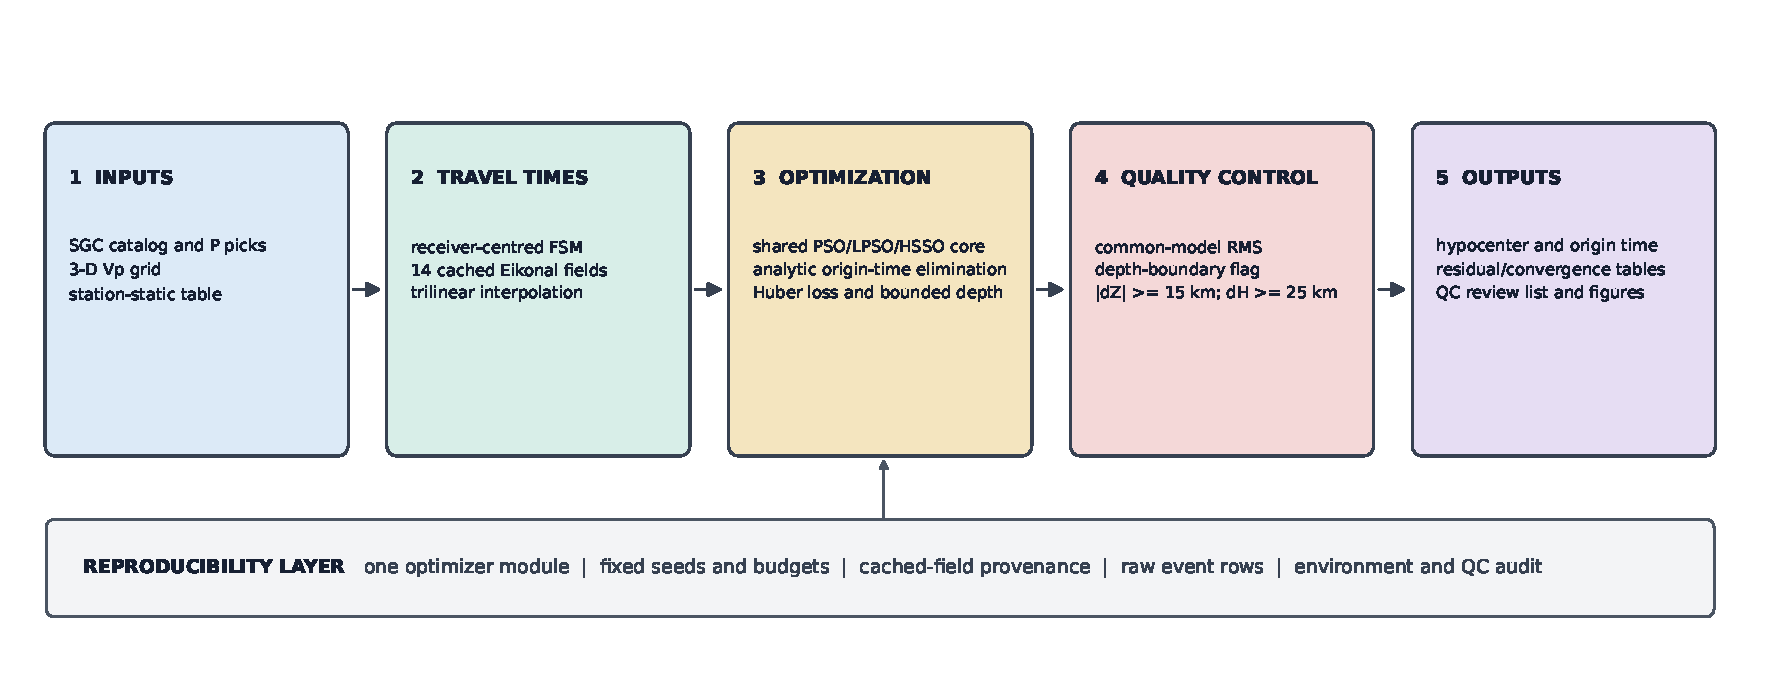
\includegraphics[width=\linewidth]{hsso_hypo_workflow.pdf}
\caption{HSSO-Hypo computational workflow. Receiver-centred FSM fields are cached once and shared by all optimizers. A single residual definition analytically eliminates origin time, and every terminal solution passes through the same displacement and boundary checks. The reproducibility layer records the implementation, seeds, budgets, field provenance, event-level outputs, environment, and audit tables.}
\label{fig:workflow}
\end{figure}

\section{Theoretical framework}

\subsection{Hypocenter objective and station statics}

For event $e$ and station $j$, the observed P-arrival time relative to the catalog origin is $d_{ej}$. Given a source $\bm{x}$, the forward model is
\begin{equation}
 d_{ej}=t_{0,e}+T_j(\bm{x};v)+s_j+\epsilon_{ej},
\end{equation}
where $T_j$ is the travel time through P-wave velocity $v(\bm{x})$, $s_j$ is a station-static correction, and $\epsilon_{ej}$ contains picking error and unresolved modelling error. For every candidate source, origin time is eliminated analytically by the robust location estimate
\begin{equation}
 \widehat{t}_{0,e}(\bm{x})=\operatorname{median}_j\{d_{ej}-T_j(\bm{x};v)-s_j\}.
\end{equation}
Residuals are $r_{ej}=d_{ej}-T_j-s_j-\widehat{t}_{0,e}$. The optimizer minimizes
\begin{equation}
 J_e(\bm{x})=\left[\frac{1}{m_e}\sum_{j=1}^{m_e} L_\delta(r_{ej})\right]^{1/2},\qquad
 L_\delta(r)=\begin{cases}r^2,&|r|\leq\delta,\\2\delta|r|-\delta^2,&|r|>\delta,\end{cases}
\end{equation}
with $\delta=1$~s. Conventional RMS is retained for reporting but not used as the optimized loss. This separation limits the leverage of an isolated poor pick without concealing its contribution to the final RMS.

\subsection{Fast-sweeping travel-time fields}

First-arrival travel time satisfies the isotropic Eikonal equation
\begin{equation}
 \|\nabla T(\bm{x})\|=\frac{1}{v(\bm{x})},\qquad T(\bm{x}_j)=0.
\end{equation}
For each unique receiver node we solve the equation on the three-dimensional grid with first-order upwind differences and alternating Gauss--Seidel sweep directions. Fast sweeping follows characteristic families efficiently and has linear complexity for common Eikonal settings \citep{Zhao2005}; factored variants improve behaviour near point sources \citep{Fomel2009}. Receiver-centred fields are valid by travel-time reciprocity and are cached once, after which each swarm evaluation requires only trilinear interpolation. All candidate and catalog hypocenters are scored with the same cached fields.

\subsection{Canonical swarm algorithms}

Let $\bm{x}_i^k$, $\bm{v}_i^k$, $\bm{p}_i^k$, and $\bm{g}^k$ denote particle position, velocity, personal best, and global best at iteration $k$. Canonical PSO uses
\begin{equation}
 \bm{v}_i^{k+1}=w_k\bm{v}_i^k+c_1\bm{r}_{1i}^k\odot(\bm{p}_i^k-\bm{x}_i^k)
 +c_2\bm{r}_{2i}^k\odot(\bm{g}^k-\bm{x}_i^k),
\end{equation}
with $w_k$ decreasing linearly from 0.9 to 0.4 and $c_1=c_2=1.7$. LPSO replaces $\bm{g}^k$ in the social term by the best personal solution among the six nearest particles in position space.

The topology-only ablation and HSSO-E combine personal, local, and global information:
\begin{align}
 \bm{v}_i^{k+1}={}&0.58\bm{v}_i^k+1.45\bm{r}_{1i}^k\odot(\bm{p}_i^k-\bm{x}_i^k)
 +1.05\bm{r}_{2i}^k\odot(\bm{\ell}_i^k-\bm{x}_i^k)\nonumber\\
 &+1.15\bm{r}_{3i}^k\odot(\bm{g}^k-\bm{x}_i^k)+\bm{h}_i^k.
\end{align}
For HSSO-no-helix, $\bm{h}_i^k=\bm{0}$. For HSSO-E, two random orthonormal directions $\bm{u}_i^k$ and $\bm{z}_i^k$ define a raw rotating direction
\begin{equation}
 \bm{e}_i^k=\cos\theta_i^k\bm{u}_i^k+\sin\theta_i^k\bm{z}_i^k.
\end{equation}
Let $\bm{\Delta}$ contain the coordinate spans. Scale dependence is removed by
\begin{equation}
 \bm{d}_i^k=\frac{\bm{\Delta}\odot\bm{e}_i^k}{\|\bm{\Delta}\odot\bm{e}_i^k\|_2},\qquad
 \bm{h}_i^k=\rho_k\bm{d}_i^k.
\end{equation}
Consequently $\|\bm{h}_i^k\|_2^2=\rho_k^2$ for every realized direction and therefore $\mathbb{E}\|\bm{h}_i^k\|_2^2=\rho_k^2$. The energy budget is distributed among dimensions instead of multiplying a common amplitude by every coordinate span. We use
\begin{equation}
 \rho_k=0.010\,\sigma_{\Omega}\,\tau_k^5
 \left[1+1.5\min\left(\tfrac{n_k^{\mathrm{stall}}}{25},1\right)\right]^{-1},
 \qquad \tau_k=1-\frac{k+1}{K},
\end{equation}
where $\sigma_{\Omega}=d^{-1}\sum_{j=1}^{d}\Delta_j$ is the scalar mean span and $n_k^{\mathrm{stall}}$ counts consecutive iterations without global improvement. Thus, raw rotating direction $\bm e_i^k$, normalized direction $\bm d_i^k$, progress fraction $\tau_k$, span vector $\bm\Delta$, mean span $\sigma_\Omega$, and stagnation count $n_k^{\mathrm{stall}}$ all have distinct symbols. The perturbation has a finite early exploration budget and is exactly zero at the last update. No gradient descent, local polishing, restart, adaptive initialization, or local-search phase is used.

The constants were fixed before any seismic evaluation in the companion algorithm-verification study \citep{Parra2026Companion}. Calibration used seeds 100--109, disjoint from the 30 evaluation seeds. Exponents 5 and 6 both obtained 10/10 successes on shifted Rastrigin 2D and Ackley 10D in calibration; exponent 5 was retained because it preserves a slightly longer exploratory phase. The scale 0.010, stagnation horizon 25, and attenuation factor 1.5 were then frozen. No earthquake or seismic residual was used for tuning.

\begin{table}[H]
\centering\small
\caption{Fixed optimizer and relocation hyperparameters. Companion-calibrated values were selected without seismic residuals; PSO values follow the canonical comparison design.}
\label{tab:parameters}
\begin{tabular}{lll}
\toprule
Component & Parameter & Fixed value\\
\midrule
All swarms & particles; updates; neighbours & $30$; $300$; $6$\\
PSO/LPSO & inertia; cognitive/social & $0.9\rightarrow0.4$; $1.7/1.7$\\
PSO/LPSO & componentwise velocity cap & $0.20\bm\Delta$\\
Topological HSSO & inertia; personal/local/global & $0.58$; $1.45/1.05/1.15$\\
Topological HSSO & componentwise velocity cap & $0.18\bm\Delta$\\
HSSO-E & scale; exponent & $0.010$; $5$\\
HSSO-E & stall horizon; attenuation & $25$; $1.5$\\
Relocation & Huber threshold; depth window & $1.0$~s; catalog $\pm20$~km\\
\bottomrule
\end{tabular}
\end{table}

\section{Materials and methods}

\subsection{Velocity model, catalog, and picks}

The application domain spans approximately $-74.60$ to $-72.55^{\circ}$ longitude and $6.20$ to $8.05^{\circ}$ latitude. The P-wave grid has 10-km spacing, 25 by 18 horizontal nodes, and 23 depth nodes from 0 to 220~km. It was obtained in the preceding MMV tomography workflow from 4,269 P picks for 913 SGC earthquakes recorded by 14 stations. The inversion used fixed catalog hypocenters, iterative slowness updates, and an active-cell coverage mask; its reported travel-time RMS decreased from 1.438 to 0.898~s. This relocation study treats that velocity volume as fixed. Fifteen of the 32 stratified events contributed picks to the velocity inversion, whereas none of the 30 new events did. The second set is therefore held out from velocity-model estimation, while the first is a stratified application set rather than an independent validation set.

Event metadata and manually reviewed solutions originate from the SGC seismicity catalog \citep{SGCCatalog}. The first evaluation set contains 32 events selected before optimizer comparison by stratifying catalog depth into 10-km intervals and retaining two eligible events per interval. The independent extension contains 30 previously unused SGC events, also depth-stratified. Events require at least four distinct P-pick stations, catalog RMS below 1~s, and source and receivers inside the model. The 32-event set is evaluated without statics. For the 30-event extension, robust receiver terms are estimated from 1,701 other events after excluding all 30 evaluation identifiers. This removes 28 overlapping events (219 picks) from the original static-training pool. A station term is retained only with at least 20 finite training events; three under-supported stations are assigned zero. Per-event median origin shifts are removed before station medians are calculated, and the supported terms are centred for identifiability. Thus, the new-event branch is held out from both the fixed velocity inversion and station-static estimation.

\subsection{Experimental design}

Mathematical verification uses shifted Rastrigin in 2 and 10 dimensions, shifted Ackley in 10 dimensions, and Six-Hump Camel in two dimensions. Thirty seeds are used per method and objective. Each run has 30 particles and 300 updates, for 9,030 objective evaluations. Success is $|f(\widehat{\bm{x}})-f^*|<10^{-6}$. The translated optima ensure that success cannot result from a hard-coded origin.

A compact source-recovery test complements the function benchmarks. Three event geometries nearest the 20th, 50th, and 80th catalog-depth percentiles are selected from each seismic data set. For each geometry, a known source is displaced by 5--10~km from the catalog point while remaining inside the same search box used for real relocation. Synthetic arrivals are sampled from the cached receiver-centred FSM fields, include the applicable held-out statics, independent Gaussian pick noise with $\sigma=0.05$~s, and zero-median receiver delays with $\sigma=0.10$~s that are not supplied to the inverse calculation. All four methods use the same noise realization, initialization, bounds, and 9,030-evaluation budget for each of the six cases. Because generation and inversion share the fixed velocity field, this experiment diagnoses conditional source and optimizer recovery under realistic station geometry; it is not an independent validation of the velocity model.

The seismic comparison imports the same \texttt{optimize()} function and immutable parameter object used by the mathematical script. For each earthquake, all methods receive the same seed, bounds, objective, and initial-position random stream. Search bounds are centred on the SGC solution, use the same geometry-dependent horizontal extent for all four methods, and restrict depth to the catalog value $\pm20$~km, clipped to the model. Velocities are clipped at 20\% of coordinate span for PSO/LPSO and 18\% for the two topological methods. Candidate positions are clipped to the common box. No post-optimization polishing is performed.

The reference ``SGC-model'' RMS is not the RMS printed in the catalog. It is recomputed at the SGC hypocenter with exactly the picks, statics, velocity model, FSM fields, and origin-time estimator used for relocation. This produces a like-for-like baseline. Primary comparisons use event-paired RMS and two-sided Wilcoxon signed-rank tests; Holm correction controls the family of six seismic pairwise tests \citep{Derrac2011}.

The Huber transition was fixed at $\delta=1.0$~s before the seismic comparison. To test whether this scale controls the reported solution, HSSO-E was replayed for all 62 events with $\delta=0.5$ and $1.5$~s while holding the seed, initialization, bounds, FSM fields, statics, and budget fixed. Sensitivity is reported as the change from the corresponding $\delta=1.0$ solution; these replays are diagnostic and were not used to select optimizer parameters.

A repeated-seed audit targeted the six largest normalized QC excursions in each data set among the 35 pre-flagged HSSO-E solutions. Excursion severity was defined as the maximum of $d_H/25$, $|d_Z|/15$, and the depth-boundary indicator. Each selected event was replayed with its original seed and nine additional predetermined seeds, while the optimizer, initialization rule, bounds, fields, statics, and 9,030-evaluation budget remained fixed. Within-event standard deviations and ranges of RMS, $d_H$, and $d_Z$, together with boundary frequencies, quantify stochastic uncertainty. Selection used only predefined QC severity and was not used to tune the optimizer.

Wall time was measured around each complete optimizer call, including initialization and all 9,030 objective evaluations with trilinear interpolation of cached FSM fields. It excludes the one-time construction or disk loading of the 14 receiver fields and excludes output serialization. Timings were obtained in a single-process Python 3.14 run on a two-core Intel Core i7-5500U (2.40~GHz) under Windows 11; they are intended for relative algorithm comparison, not as hardware-independent performance claims.

\subsection{Quality control and reproducibility}

Three flags are defined before inspecting optimizer outcomes: (i) a relocated depth within the larger of 0.25~km or 1\% of the vertical interval from a bound, (ii) horizontal displacement $d_H\geq25$~km, and (iii) absolute vertical displacement $|d_Z|\geq15$~km. Flagged events are not deleted from the statistical comparison. They are reported separately because a boundary optimum or a large displacement may indicate inadequate illumination, a residual velocity error, an erroneous pick, or a search interval that truncates the solution.

The compendium records software environment, random seeds, immutable optimizer parameters, input checksums, selected catalog rows, P picks, statics, velocity-grid metadata, cached FSM fields, raw per-event output, convergence histories, analysis scripts, and manuscript figures. The optimizer exists in one shared module rather than copied benchmark and relocation implementations. The release at \url{https://github.com/romusan/hsso-hypo-reproducibility} uses the OSI-approved MIT licence and includes a dependency-light executable example, invariant checks, and a SHA-256 manifest. A permanent archive identifier will be added before submission, consistent with the code and reproducibility policy of \textit{Computers \& Geosciences}.

\section{Results}

\subsection{Mathematical verification}

Figure~\ref{fig:validation}a reports success counts for the four benchmark functions. All methods succeeded in 30/30 runs on shifted Rastrigin 2D and Six-Hump Camel except HSSO-no-helix, which succeeded in 27/30 Rastrigin runs. On Ackley 10D, PSO and HSSO-no-helix succeeded in 30/30 runs, HSSO-E in 29/30, and LPSO in 5/30. None of the methods met the $10^{-6}$ criterion on Rastrigin 10D; median objective errors were 6.47 (PSO), 10.28 (LPSO), 11.94 (no helix), and 13.93 (HSSO-E). This failure is retained as a scope limitation and directly contradicts a universal-superiority interpretation.

\begin{figure}[t]
\centering
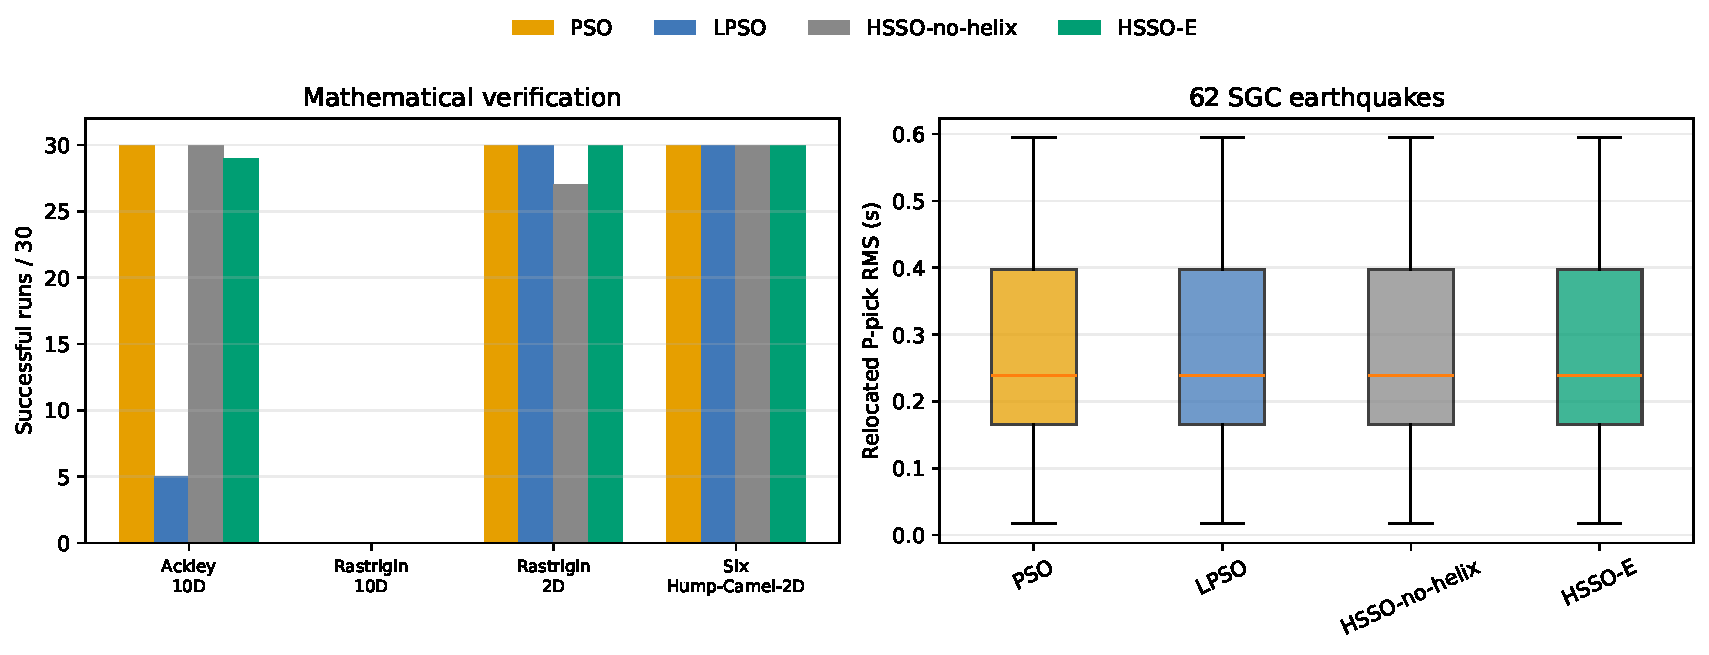
\includegraphics[width=\linewidth]{algorithm_and_seismic_validation.pdf}
\caption{(a) Mathematical verification with 30 paired seeds and 9,030 evaluations per run. (b) Event-wise P-pick RMS for the four shared-core optimizers across 62 earthquakes. Boxes show medians and interquartile ranges; whiskers follow the standard 1.5-IQR convention and plotted outliers are suppressed for legibility but retained in all tables and tests.}
\label{fig:validation}
\end{figure}

\subsection{Compact synthetic recovery}

All four methods converged to the same recovered source to the precision shown in Table~\ref{tab:synthetic}. Across the six geometries, median horizontal, absolute-depth, and three-dimensional errors were 1.02, 2.44, and 2.67~km, respectively; four sources were recovered within 5~km and the maximum three-dimensional error was 5.97~km. The two errors above 5~km occurred in intermediate-to-deep cases and were dominated by depth (5.77 and 5.91~km), while horizontal errors remained below 1.50~km in every case. This small experiment demonstrates conditional numerical recovery in the adopted model and shows again that the terminal basin, rather than optimizer identity, controls the final solution. It does not test errors in the velocity field or establish real-event accuracy.

\begin{table}[H]
\centering\small
\caption{Compact synthetic recovery using six real station geometries, $\sigma=0.05$~s pick noise, and unmodelled zero-median receiver delays with $\sigma=0.10$~s.}
\label{tab:synthetic}
\begin{tabular}{lrrrrr}
\toprule
Method & Median $e_H$ & Median $|e_Z|$ & Median $e_{3D}$ & Max. $e_{3D}$ & $N_{e_{3D}\leq5}$\\
 & (km) & (km) & (km) & (km) & /6\\
\midrule
PSO & 1.02 & 2.44 & 2.67 & 5.97 & 4\\
LPSO & 1.02 & 2.44 & 2.67 & 5.97 & 4\\
HSSO-no-helix & 1.02 & 2.44 & 2.67 & 5.97 & 4\\
HSSO-E & 1.02 & 2.44 & 2.67 & 5.97 & 4\\
\bottomrule
\end{tabular}
\end{table}

\subsection{Seismic relocation and ablation}

The shared-data comparison evaluates 32 depth-stratified events and 30 held-out SGC events. Mean RMS decreased from 0.631 to 0.367~s in the stratified set and from 0.596 to 0.230~s in the held-out set; every event improved relative to its strictly comparable catalog baseline. Table~\ref{tab:seismic} shows nearly identical rounded aggregates across methods. This is not a transcription artifact: an event-wise audit found RMS ranges below $10^{-10}$~s for 44/62 events, locations within 1~m for 53/62, and locations within 100~m for 58/62. Four events had larger spatial differences. The largest RMS spread occurred for SGC2025pgzatv ($1.07\times10^{-4}$~s), with 0.99~km horizontal and 1.62~km depth spread among methods; none of its solutions touched a bound. Event-paired HSSO-E comparisons found no significant difference after Holm correction (all adjusted $p=1$); matched-pairs rank-biserial effects ranged from $-0.212$ to $0.099$, where negative values favour HSSO-E, and are consistent with small effects. The near-perfect agreement indicates that, for this model and data geometry, the objective is sufficiently smooth for all tested swarms to reach the same basin in most events. It also underscores that residual reduction alone cannot validate absolute-location improvement.

Convergence histories nevertheless distinguish search dynamics. The median iteration at which the best objective came within $10^{-4}$~s of its final value was 65.5 (PSO), 78.5 (LPSO), 18.5 (HSSO-no-helix), and 23.5 (HSSO-E) for the stratified set; corresponding values for the 30 new events were 65.0, 77.5, 19.0, and 33.5. Topological guidance accelerated convergence relative to PSO/LPSO, but the helical perturbation delayed final refinement relative to the no-helix ablation. This is evidence for the topological component, not for a positive helical effect in the present seismic objective.

Runtime does not follow iteration-to-tolerance alone (Table~\ref{tab:runtime}). Across the 62 full-budget runs, pooled median optimizer times were 0.675~s for PSO, 1.016~s for LPSO, 1.484~s for HSSO-no-helix, and 1.464~s for HSSO-E. A deterministic replay stopped each method when its best objective first came within $10^{-4}$~s of that method's full-budget terminal value. HSSO-E then required a median of 765 evaluations rather than PSO's 2,085 and reduced pooled wall time from 0.157 to 0.136~s. HSSO-no-helix was fastest at 600 evaluations and 0.107~s. The result is data-set dependent: HSSO-E was faster than PSO for the 30 held-out events (0.127 versus 0.159~s) but slightly slower for the stratified set (0.162 versus 0.149~s). Thus, topology improves evaluation efficiency and can enable earlier diagnostics, while the helical term does not provide a uniform wall-time advantage.

The full-budget relative penalty is substantially smaller than in the companion analytical benchmarks \citep{Parra2026Companion}: HSSO-no-helix required 12.6--14.9 times the PSO time and HSSO-E required 15.9--19.9 times, compared with 2.20 and 2.17 here. This ratio compression is consistent with the complexity model $O(NC_f+N^2d)$: cached FSM interpolation increases the common objective cost $C_f$, diluting the relative contribution of neighbour search and orthonormal-plane generation. Because the two timing studies were separate execution sessions, the comparison supports this computational interpretation but is not presented as a portable hardware speedup.

\begin{table}[H]
\centering\small
\caption{Full-budget and early-stop optimizer cost pooled across 62 events after FSM fields were cached. Early stopping targets an objective within $10^{-4}$~s of each method's own terminal value.}
\label{tab:runtime}
\begin{tabular}{lrrrrr}
\toprule
Method & Full time (s) & Early iter. & Early eval. & Early time (s) & Relative\\
\midrule
PSO & 0.675 & 68.5 & 2,085 & 0.157 & 1.00\\
LPSO & 1.016 & 78.0 & 2,370 & 0.270 & 1.72\\
HSSO-no-helix & 1.484 & 19.0 & 600 & 0.107 & 0.68\\
HSSO-E & 1.464 & 24.5 & 765 & 0.136 & 0.87\\
\bottomrule
\end{tabular}
\end{table}

\begin{table}[H]
\centering\small
\caption{Seismic validation summary from one terminal solution per event and method. Mean RMS is averaged over events; displacement columns are event medians. Values are rounded to the shown precision. $N_b$ denotes depth-boundary solutions and $N_{25}$ denotes horizontal displacements of at least 25~km.}
\label{tab:seismic}
\begin{tabular}{llrrrrr}
\toprule
Data set & Method & Events & Mean RMS (s) & Median $d_H$ (km) & Median $|d_Z|$ (km) & $N_b/N_{25}$\\
\midrule
32 stratified & PSO & 32 & 0.367 & 6.88 & 13.71 & 12/1\\
32 stratified & LPSO & 32 & 0.367 & 6.88 & 13.71 & 12/1\\
32 stratified & HSSO-no-helix & 32 & 0.367 & 6.88 & 13.71 & 12/1\\
32 stratified & HSSO-E & 32 & 0.367 & 6.88 & 13.71 & 12/1\\
30 held out & PSO & 30 & 0.230 & 10.50 & 14.81 & 9/4\\
30 held out & LPSO & 30 & 0.230 & 10.50 & 15.62 & 9/4\\
30 held out & HSSO-no-helix & 30 & 0.230 & 10.50 & 15.55 & 9/4\\
30 held out & HSSO-E & 30 & 0.230 & 10.50 & 15.40 & 9/4\\
\bottomrule
\end{tabular}
\end{table}

\subsection{Quality-control outcomes}

Figure~\ref{fig:qc} separates residual reduction from displacement diagnostics for HSSO-E. All points lie below the identity line, but 12 stratified and 9 held-out solutions touch a depth boundary; 1 and 4 events, respectively, exceed the 25-km horizontal threshold. The union of boundary, horizontal, and vertical flags contains 15 of 32 and 20 of 30 events. These cases are not automatically incorrect, but their frequency prevents interpreting the RMS reduction as a validated improvement in absolute location. The 35 flagged HSSO-E events and individual reasons are provided in the supplementary event table.

\begin{figure}[t]
\centering
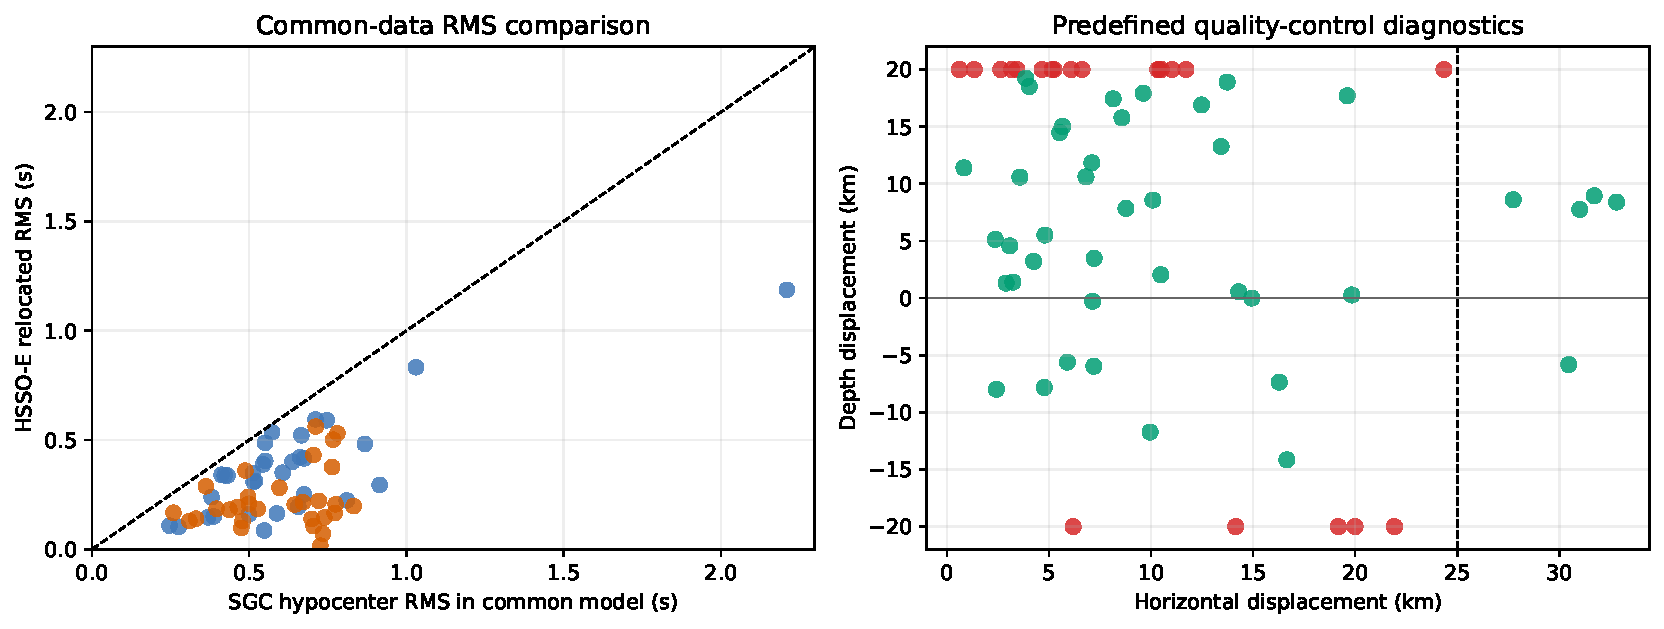
\includegraphics[width=\linewidth]{hsso_e_relocation_qc.pdf}
\caption{HSSO-E seismic validation. Left: RMS at the catalog hypocenter and after relocation, evaluated with identical data and forward model. Right: horizontal and vertical displacements; red indicates a depth-boundary solution and the dashed line is the $d_H=25$~km review threshold.}
\label{fig:qc}
\end{figure}

\subsection{Repeated-seed sensitivity}

The 120-run audit found negligible stochastic dispersion in the 12 difficult, pre-flagged events (Table~\ref{tab:seeds}). The largest horizontal range across 10 seeds was 0.00246~km (2.46~m), the largest depth-shift range was $4.59\times10^{-8}$~km, and no event changed depth-boundary status. The original-seed rows reproduce the main analysis. These results separate numerical repeatability from geophysical validity: seed stability does not remove a QC flag or demonstrate that a boundary solution is physically correct.

\begin{table}[H]
\centering\small
\caption{Within-event HSSO-E dispersion for 12 pre-flagged events replayed with 10 seeds each.}
\label{tab:seeds}
\begin{tabular}{lrrrr}
\toprule
Quantity & Median SD & Maximum SD & Median range & Maximum range\\
\midrule
RMS (s) & $3.61\times10^{-15}$ & $4.89\times10^{-8}$ & $1.02\times10^{-14}$ & $1.62\times10^{-7}$\\
$d_H$ (km) & $9.44\times10^{-7}$ & $8.42\times10^{-4}$ & $2.94\times10^{-6}$ & $2.46\times10^{-3}$\\
$d_Z$ (km) & 0 & $1.44\times10^{-8}$ & 0 & $4.59\times10^{-8}$\\
\bottomrule
\end{tabular}
\end{table}

\subsection{Robust-loss sensitivity}

Table~\ref{tab:huber} shows that relaxing the Huber transition from 1.0 to 1.5~s leaves the median solution effectively unchanged in both data sets. The largest depth change was 0.57~km in the held-out set; one stratified event changed by more than 1~km. The more aggressive $\delta=0.5$~s transition affected a minority of events: 3/30 held-out and 7/32 stratified solutions changed depth by more than 1~km, with maxima of 4.92 and 8.93~km. Median RMS change remained below numerical reporting precision for the held-out events and was $8.0\times10^{-4}$~s for the stratified set, but four and nine individual events, respectively, changed by more than 0.01~s. The main $\delta=1.0$ results are therefore stable to an upward relaxation and conditionally robust, rather than invariant, to stronger downweighting of large residuals.

\begin{table}[H]
\centering\small
\caption{HSSO-E sensitivity to the Huber transition relative to the fixed $\delta=1.0$~s analysis. $N_{|\Delta z|>1}$ counts events whose relocated depth changes by more than 1~km.}
\label{tab:huber}
\begin{tabular}{llrrr}
\toprule
Data set & $\delta$ (s) & Median $|\Delta\mathrm{RMS}|$ (s) & $N_{|\Delta z|>1}$ & Max. $|\Delta z|$ (km)\\
\midrule
32 stratified & 0.5 & $8.0\times10^{-4}$ & 7 & 8.93\\
32 stratified & 1.5 & $<10^{-12}$ & 1 & 3.58\\
30 held out & 0.5 & $<10^{-12}$ & 3 & 4.92\\
30 held out & 1.5 & $<10^{-12}$ & 0 & 0.57\\
\bottomrule
\end{tabular}
\end{table}

\section{Discussion}

\subsection{What the helical energy control does---and does not establish}

The energy formulation resolves a dimensional ambiguity in coordinate-wise helical amplitudes. Multiplying one amplitude by every coordinate span makes total perturbation energy grow with dimension and anisotropy. Normalizing the span-weighted direction first and assigning $\rho_k$ afterwards fixes the squared norm exactly. This permits an auditable statement about the exploration budget and makes the same rule meaningful for dimensionless test functions and kilometre-scale hypocenters.

The helical term should not be interpreted as guaranteed escape from every local minimum. Its practical role is narrower: early rotating perturbations diversify directions around personal, neighbourhood, and global attractors; the topology preserves multiple channels of information; and the energy decays so the final iterations are not dominated by artificial motion. The experiments show both sides of that trade-off. HSSO-E recovered three Rastrigin-2D runs missed by the no-helix ablation, but it was less reliable on Ackley 10D, failed with all methods on Rastrigin 10D, and converged more slowly than the no-helix method in the seismic objective. Whether the perturbation helps depends on landscape and budget, as expected from no-free-lunch results \citep{WolpertMacready1997}.

\subsection{Geophysical interpretation and station terms}

An RMS decrease means that the relocated point is more compatible with the selected P picks under the adopted velocity model and station corrections. It does not by itself prove that the hypocenter is closer to the physical rupture nucleation point. The velocity volume was inverted using fixed SGC locations; reusing it for relocation introduces a dependency that should be acknowledged. Large shifts may absorb smooth velocity bias, while station statics may absorb unresolved receiver-side structure. Conversely, omitting statics can force the source coordinates to explain systematic station delays. The separate 32- and 30-event branches make that distinction traceable.

Regional context supports the need for this caution. The MMV contains shallow low-velocity basin structure \citep{Londono2020}, and ambient-noise results reveal pronounced variations across the Colombian Andes \citep{Poveda2018}. A 10-km grid cannot represent all near-surface or fault-zone structure. Station corrections are consequently defensible nuisance parameters, but their provenance and sign convention are part of the scientific model. Here, all 30 evaluation identifiers are excluded before the robust station medians are estimated, and under-supported receivers are explicitly assigned zero rather than unstable corrections.

An exploratory geometry check does not support a simple geological explanation for all flagged solutions. In the stratified set, flagged events are deeper than unflagged events in median catalog depth (109.7 versus 46.8~km) and have slightly fewer stations (8 versus 9); horizontal displacement is inversely associated with station count (Spearman $\rho=-0.44$, $p=0.011$). In the held-out set, flagged events have larger median horizontal displacement (12.1 versus 7.0~km), but displacement has no significant rank association with station count, catalog gap, or depth. These post-hoc diagnostics suggest an illumination component, but no claim of correlation with a basin edge or fault is made without an explicit geological-distance test.

\subsection{Comparison with established relocation strategies}

HSSO-Hypo addresses a different use case from double-difference relocation. Double difference exploits correlated paths between nearby events and is preferable when dense clusters and reliable differential times exist \citep{WaldhauserEllsworth2000}. NonLinLoc-type methods estimate a location probability density and are preferable when calibrated uncertainty is the principal output \citep{Lomax2000}. The present framework supplies a bounded robust optimum and convergence diagnostics, not a posterior distribution. Its value is modularity: the same FSM fields and residual definition can support future uncertainty sampling or a differential-time objective without claiming that the swarm replaces those methods.

A compact external-method pilot was also performed on the same 62-event catalog. NonLinLoc returned 62 P-only absolute solutions in a layered MMV model (median RMS 0.170~s); median catalog-to-solution shifts were 8.29~km horizontally and 12.27~km vertically, of the same broad order as the conditional HSSO-E shifts. These numbers are not a ranked benchmark because the pilot used a one-dimensional model, a different residual formulation, and no matched $\pm20$~km depth window. Differential times constructed with \texttt{ph2dt} linked 56 events through 520 catalog-P pairs in eight clusters. HypoDD retained 56, 48, and 10 events under progressively different reweighting and pruning schedules, demonstrating material schedule sensitivity. No waveform cross-correlation times were used. The pilot therefore functions as an external diagnostic and a reproducible starting point for a future matched-design comparison, not as evidence that one relocation family wins.

\subsection{Limitations and next validation steps}

Five limitations bound the current conclusions. First, relocation is conditional on a fixed velocity field originally inverted with catalog hypocenters. Source and slowness errors are covariant, so a source displacement can compensate a velocity anomaly and a lower conditional RMS cannot establish a more accurate absolute hypocenter. The 30 new events are excluded from that velocity inversion, but they remain subject to regional model bias; the 32-event set includes 15 events that contributed picks to the model and is interpreted only as a stratified application set. A joint source--velocity inversion, an ensemble of plausible velocity fields, or cross-validated models is required to quantify this covariance. The compact synthetic test shares the forward and inverse velocity field and contains only six geometries; its added noise and receiver delays prevent exact inversion, but it remains an algorithmic recovery check rather than independent geophysical validation. Second, real-event accuracy cannot be measured without independent ground truth such as quarry blasts, dense temporary arrays, or high-precision relative locations. Third, the repeated-seed audit establishes numerical stability for 12 difficult events, not all 62, and cannot resolve velocity-model or search-bound uncertainty. Fourth, the depth window can create boundary optima, which are reported rather than silently accepted. Fifth, the held-out station terms remove direct evaluation-event leakage but remain conditional estimates from catalog sources and a fixed forward model; three poorly sampled receivers require zero rather than estimated corrections.

A strong next experiment is a synthetic recovery test using the actual station geometry and velocity grid: generate arrivals from off-catalog sources, add controlled picking noise and withheld station delays, and compare coordinate error rather than only residual. A checkerboard-style collection of sources across well- and poorly-illuminated cells would show where each optimizer can recover depth and where the data geometry makes the inverse problem non-identifiable.

\section{Conclusions}

HSSO-Hypo establishes a reproducible architecture for conditional hypocenter relocation in a three-dimensional regional model. The same source file implements PSO, LPSO, HSSO-no-helix, and HSSO-E in mathematical and seismic experiments, eliminating an important source of methodological drift. Receiver-centred FSM fields, robust analytical origin-time elimination, held-out station statics, bounded depth, and predefined displacement flags connect the optimizer to an auditable geophysical workflow. In the present data, all four optimizers reach effectively the same final RMS, demonstrating that the forward model and data geometry dominate the terminal basin. Topological guidance substantially reduces evaluations to that basin and, under a reproducible early-stop rule, reduces pooled wall time; the no-helix ablation remains the fastest configuration. The repeated-seed audit shows that the difficult HSSO-E solutions are numerically stable while leaving their geophysical QC status explicitly unresolved.

The framework's most important scientific output is not the smallest RMS in isolation. It is the paired record linking every residual change to a fixed forward model, common picks, explicit corrections, a reproducible random state, a search boundary, and a quality-control decision. That record makes improvements testable and questionable relocations visible, which is the basis required for defensible application to the Middle Magdalena Valley and for extension to other regional networks.

\section*{Code and data availability}
The release package contains the canonical optimizer module, FSM relocation and analysis scripts, environment specification, selected SGC event metadata and picks subject to source terms, station-static table, velocity grid, cached receiver fields, configuration files, raw results, checksum manifest, and minimal examples. It also archives all 120 repeated-seed rows and their configuration, the six paired-test rows with raw and Holm-adjusted $p$ values and rank-biserial effects, the 35-event QC supplement, and the NonLinLoc/HypoDD pilot configurations and summary outputs. A dependency-light audit verifies these claimed contents and their SHA-256 checksums. Software is licensed under the OSI-approved MIT licence; SGC-derived inputs retain their source terms. The versioned public repository is available at \url{https://github.com/romusan/hsso-hypo-reproducibility}; a permanent archive identifier will be added before submission. The authoritative earthquake metadata source is the Servicio Geol\'ogico Colombiano catalog \citep{SGCCatalog}.

\section*{Declaration of competing interest}
The author declares no known competing financial interests or personal relationships that could have appeared to influence the work reported in this paper.

\section*{Acknowledgements}
The author acknowledges the Servicio Geol\'ogico Colombiano for earthquake catalog and phase information used in this study.

\bibliographystyle{unsrtnat}
\bibliography{references}
\end{document}
